


\paragraph{Historique} 

Docteur en médecine et spécialiste en en oto-rhino-laryngologie et
neurophysiologie auditive, A. Tomatis a étudié la relation
existant entre l'oreille et la voix, et par extension entre l'écoute
et la communication en créant 
une nouvelle discipline, l'audio-psycho-phonologie, ses recherches et
découvertes furent établies au
laboratoire de physiologie de la Sorbonne et donnèrent lieu à des
communications à l'Académie des Sciences et à L'Académie de Médecine
de Paris en 1957 et 1960. Son \oe uvre représente plusieurs dizaines
de publications ainsi que treize ouvrages\footnote{Cf. la bibliographie.}.

\section{Définition de sa méthode} 

\emph\textbf{{L'audio-psycho-phonologie}}
est une pédagogie et une thérapie de l'écoute (l'audio (oreille) la psychologie et la phonologie (voix)).
 L'outil est un appareil électronique appelé
\label{outil_oreille_electro}
Oreille Electronique avec  l'utilisation d'une technique, la 
bascule, qui permet de créer une alternance entre deux conditions perceptives 
du même message sonore avec un passage soudain et imprévu de fréquences graves à des 
fréquences aiguës. Cette façon de travailler permet au
cerveau d'améliorer naturellement \emph{l'interprétation du message
sensoriel}.




Tomatis était un personnage qui s'interrogeait beaucoup  et remettait
souvent en question les théories appliquées. Il suivait son intuition
en créant ainsi 
des liens entre les disciplines avec pour motivation primordiale
l'application clinique de ses recherches. 

Il a énoncé les lois qui constituent ``l'effet Tomatis'' : 
\begin{itemize}
	\item La voix ne contient que ce que l'oreille entend.
	\item Si l'on modifie l'audition, la voix est immédiatement et 
inconsciemment
		modifiée.
	\item Il est possible de transformer la phonation par une stimulation 
auditive
		entretenue pendant un certain temps (loi de rémanence).
\end{itemize}

Il y a une action simultanée sur trois fonctions essentielles de l'oreille
: l'audition, l'équilibre et la dynamisation.
\begin{itemize}
	\item Audition : lorsque l'on s'entend, on peut mieux se structurer.
	\item Réharmonisation : équilibre et coordination : le SNC (système 
nerveux
		central) est touché lors de l'écoute de musique par 
l'intermédiaire
		du vestibule. Il y a une action sur les troubles psychomoteurs, 
les
		réponses motrices deviennent plus fluides. Les 
dysfonctionnements
		correspondent à un état de non-équilibre neurophysiologiques 
plus
		ou moins prononçés. 
	\item Stimulation : dynamiser le cerveau par des fréquences spécifiques
          et par là-même le corps tout entier.

 
\end{itemize}



Cette méthode répond ainsi à des objectifs éducatifs et rééducatifs et
est similaire à l'interdisciplinarité  que l'on retrouve
aujourd'hui dans le domaine de la 
psycho-neuro-immunologie,
(PNI) devenue actuellement discipline médicale de pointe.\footnote{La PNI étudie 
l'impact des événements psychiques sur le système immunitaire. Elle repose sur 
la mise en évidence d'interrelations entre le système
nerveux central, le système neuroendocrinien et le système immunitaire.
C'est une approche interdisciplinaire incorporant des données de la
psychologie, de la neuroscience, de la neurologie, dont l'endocrinologie
et l'immunologie. (entre autres) Source : Wikipédia, février 17.}
Sa conception est une conception intégrative
de l'homme, mettant en interaction toutes ses dimensions corporelles
et psychologiques dont 
les émotions et les cognitions.






\emph{\textbf{Conception différente de la physiologie auditive}}

Tomatis  s'oppose sur plusieurs points à G. Békésy\footnote{Georg Békésy, prix 
Nobel de physiologie 1961, l'oreille ne sert qu'à transmettre les sons de manière passive
comme peut le faire un micro et le rôle des osselets 
se limite à la transmission du
son. }  au sujet de la
physiologie auditive, qu'il considère comme active et non passive. \footnote{Cf. Annexe sur l'anatomie de l'oreille et sa physiologie}


\begin{itemize}
	\item l'oreille moyenne et son rôle de transmetteur 
	\item l'analyse fréquentielle au niveau de la cochlée
\end{itemize}

Son originalité réside dans sa conception de la transmission du son
au niveau de l'oreille interne. 

\emph{Un organe actif}

Il propose une nouvelle compréhension de l'oreille, celle-ci étant,
à son regard, un organe \emph{actif} % j'ai souligné
dans le sens suivant :
\begin{itemize}
	\item L'oreille moyenne, grâce aux muscles de l'étrier et du marteau, 
fait
		un\textbf{ travail de visée} en ciblant les sons à écouter : le tympan 
se tend
		pour se mettre en résonance avec les sons à percevoir.
	\item Il fait aussi un autre travail qui est celui de \textbf{sélectionner des 
sons
		pour se protéger} : la tension tympanique se détend pour amortir 
l'intensité
		sonore qui inonde l'oreille interne. 
\end{itemize}




\begin{figure}
	\centering
	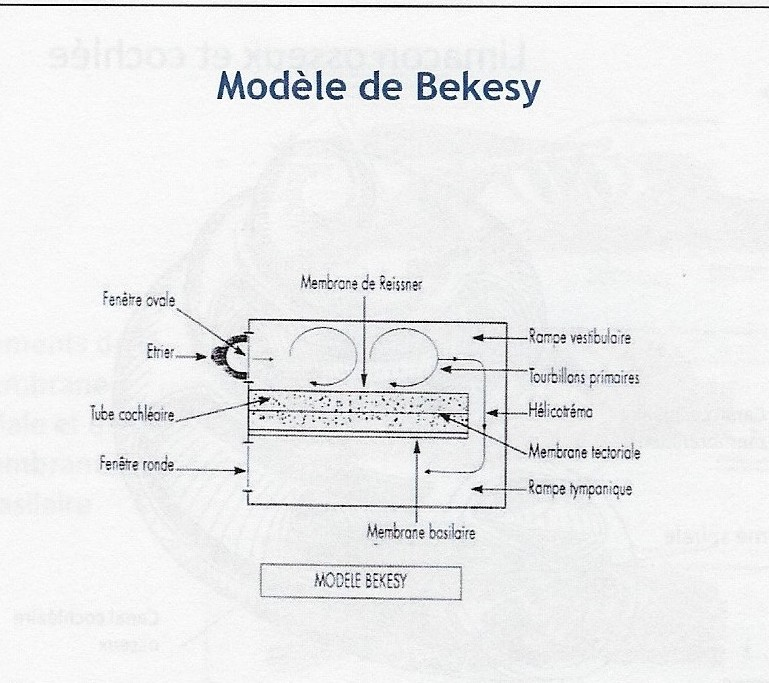
\includegraphics[width=0.7\linewidth]{images/Cochleederoule_bas.jpg}
	\caption[Modèle de Békésy]{Modèle de Békésy}
	\label{fig:cochleederoulebas}
\end{figure}


 


\begin{figure}
	\centering
	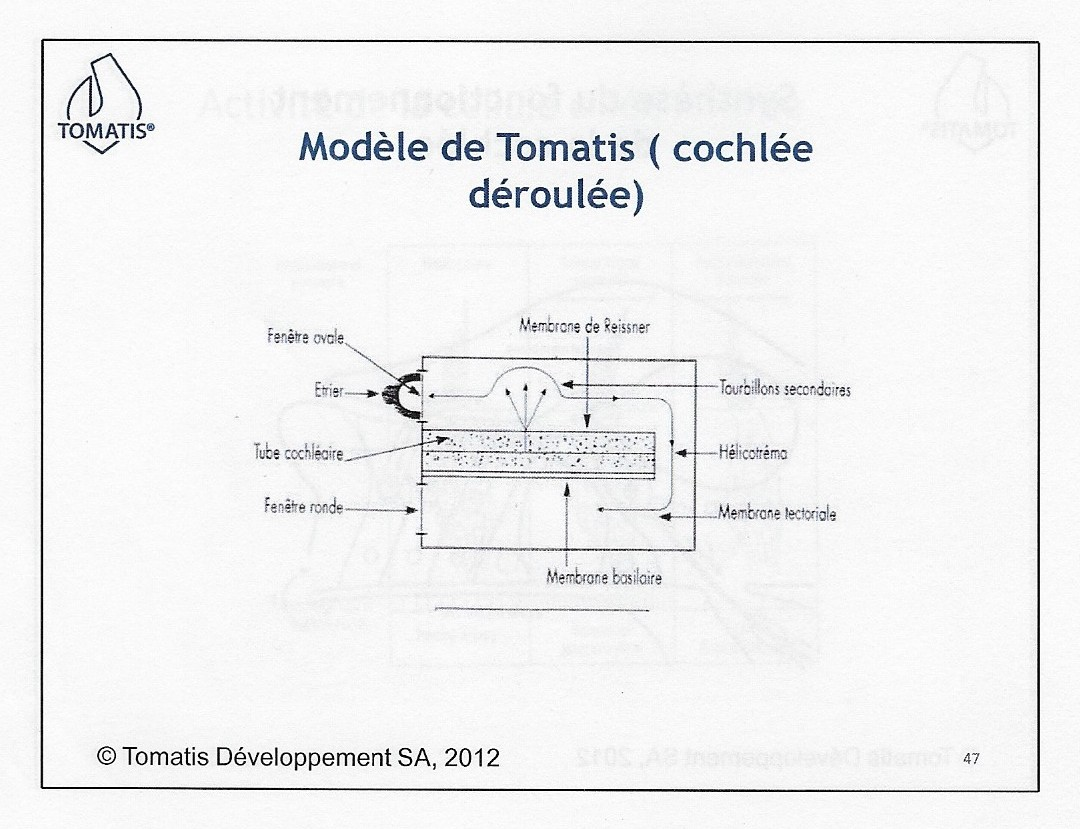
\includegraphics[width=0.7\linewidth]{images/Cochleederoule_haut.jpg}
	\caption[Cochlée selon Tomatis]{Cochlée selon Tomatis}
	\label{fig:cochleederoulehaut}
\end{figure}


D'après son hypohèse, \footnote{Conférence au IIème Congrès International d'Audio-Psycho-Phonologie
Paris 1972:  \emph{Nouvelles théories sur la physiologie auditive}.}.
 les sons arrivent bien par le canal auditif
jusqu'au tympan. L'onde acoustique excite la membrane tympanique et
par voie de conséquence, l'os de la caisse du tympan. 
A l'instar d'une
peau de tambour qui fait chanter le bois auquel elle est attachée,
c'est toute la boîte crânienne qui inondée de sons et en particulier
l'oreille interne. Celle-ci, de par sa grande densité, capte les sons
et résonne comme du cristal\footnote{La transmission du son par l'os est de 
5000 $m/s$.}.

Les fréquences qui forment les sons vont ainsi exciter les cellules
ciliées qui tapissent la cochlée, tel un piano enroulé.

{\textbf{L'analyse multifréquentielle ne se pose plus} 
avec sa théorie: chaque fréquence se dirige instantanément et
naturellement vers la cellule ciliée qui lui correspond. 
C'est grâce à la forme particulière du limaçon qu'il y a un tri fréquentiel 
instantané.
Le son de fréquence identique s'installe toujours au même endroit, sur une 
ligne isofréquentielle, qui est une tranche perpendiculaire à l'axe.
Le rôle des tourbillons est de s'adapter aux bruits
et non de transmettre les sons.
Lorsque l'intensité des sons aug\-men\-te,
l'ex\-ci\-ta\-tion des cellules ciliées provoque des perturbations liquidiennes
dans l'oreille interne, c'est-à-dire des tourbillons. Ceux-ci se propagent
et sont amortis par l'étrier. Si les sons atteignent une intensité
dangereuse pour les cellules ciliées, l'étrier réagit fortement et
entraîne une réaction du marteau qui modifie la tension du tympan.
A son tour, le tympan, relâché, amortit le volume sonore transmis
à l'oreille interne, comme la paupière qui se ferme quand la lumière
est trop intense.


\begin{quotation}
	Le tympan se met dans un certain état de tension pour jouer le
	rôle d'un diapason qui fait vibrer toute la boîte crânienne
	par l'intermédiaire du \emph{sulcus tympani}. 
	\emph{C'est toute la boîte crânienne qui vibre et qui transmet le son à 
la vésicule labyrinthique et non à la chaîne ossiculaire que l'on a l'habitude 
de considérer comme le véhicule du son.} La chaîne ossiculaire est un ensemble 
qui
	joue le rôle d'adaptateur, de régulateur et non de transmetteur. La
	conduction du son par l'air puis par l'os doit donc
	être étudiée d'une façon complémentaire afin que l'on
	puisse déterminer par la suite la posture d'écoute du sujet%
	\footnote{Entretien réalisé par B. Auriol avec Tomatis, Anvers 
1973.}.\pdfmargincomment{quel livre?}

\end{quotation}


 Notons que le  rôle important et
particulier 
de la \textbf{cochlée} sur notre audition fait encore à l'heure
actuelle l'objet de recherches intenses
par l'équipe de Christine Petit qui relève
son aspect encore très mystérieux:

\nomenclature{cochlée}{Anatomie : organe de l'audition, appareil sensoriel, 
en forme de spirale, la cochlée, incluse dans l'os du rocher, 
forme le limaçon membraneux, se situe dans l'oreille interne et 
permet de déceler des sons extrêmement faibles, de discréminer des fréquences
et de masquer des sons faibles par des sons forts.}
<<\,C'est une sorte de minuscule appareil électroacoustique capable
de discréminer des sons extrêmement faibles, capable de \emph{masquer
les sons faibles par des sons forts}, pouvant \emph{distordre les
sons,} et en conséquent, \emph{capable d'élaborer un traitement extrêmement
sophistiqué des sons}%
% OGA: référence stp. Salters et Gaullier ont publié? émission?
\footnote{Christine Petit, titulaire de la chaire Génétique et
physiologie cellulaire au Collège de France, entretien en novembre 2012, 
réalisé par Laurent Salters et Vincent Gaullier, 
Look at science : le système sensoriel auditif confirme 
lors d'un entretien réalisé en 2012 le rôle indéniable de la cochlée.\,>>}.



 
 

 A partir des publications, études et recherches récentes \footnote{\emph{Tomatis Research and Publication} www.tomatisassociation.org}    faites sur la
 méthode Tomatis, nous avons notamment
 relevé celles du Dr. med. Inge Flehming, neurologue et 
pédiatre,\footnote{Dr. med. Inge Flehming,
	neurologue, neuropédiatre, texte publié en allemand
	en 1996, \emph{``Grundsatz-Gutachten zur Behandlungsmethode
		nach Prof. Tomatis''}. Voir 
\href{http://www.analytische-hoertherapie.de/uploads/tx\_templavoila/Grundsatzgu
tachten\_zur\_Behandlungsmethode\_nach\_Prof.\_Tomatis.pdf}{le site web.}}
 , celles du Docteur Du Plessis (études sur l'anxiété en
 milieu scolaire et universitaire) qui  attestent de la pertinence de ce
 concept et de cette forme de pédagogie. \footnote{Troubles 
psychologiques : Etude du Plessis (Université de Potchefstroon
- Afrique du Sud).}  \footnote{Du même auteur, une autre étude démontre qu'après 14,3
mois le niveau d'an\-xié\-té avait continué à baisser fortement
pour le groupe Tomatis alors qu'aucun
changement n'apparaissait pour le groupe contrôle}%
\footnote{Du Plessis W. F. and Van Jaarsveld, P. E. (1988),
	``Audio-psycho-phonology : A comparative outcome study on anxious 
primary school pupils'',  Afr. Tydskr. Sielk. 1988,
	18 (4) 144--151. Du Plessis, W.F., Burger, S. (2001) [\ldots]
	\emph{A pilot study involving the Tomatis method.}, Sud Africa J. 
Psychol.}
 
En outre, cette étude pilote sur l'effet de 
--- la bascule \label{bascule} électronique qui a pour objectif de stimuler le cerveau en lui 
permettant de capter plus facilement les sons---du Dr. Carlos Escera
de l'Université de Barcelone en 2014, menée en collaboration avec le CNRS  a fait 
l'objet d'une validation
par un comité de lecture scientifique et a prouvé la stimulation
apportée au cerveau pour la captation des sons.
%
\footnote{%
\href{http://tomatisassociation.org/scientific-validation-of-the-tomatis-effect-
eeg-recordings-of-sound-from-brainstem-to-cerebral-cortex-encoding-university-of
-barcelona-2014/}{tomatisassociation.org}.}  \label{bascule}\footnote{La bascule permet 
de créer une alternance entre deux 
conditions perceptives du même message sonore: passage soudain et imprévu de 
fréquences graves à des fréquences aigües.}
En conclusion, selon Pierre Lane, journaliste de l'é\-mi\-s\-sion Envoyé 
spécial%
\autocite{tomatis_methode_1991}, Tomatis
a inventé une méthode peut-être critiquée mais qui a donné des
résultats. Elle ouvre l'oreille par des procédés mécaniques pour atteindre
des domaines spécialisés, que ce soit en médecine, en psychologie,
en ostéopathie.


\textbf{Technique de travail sous ``Oreille électronique''}}
Le but de cet appareil 
est de modifier la manière d'entendre. On obllige l'oreille à utiliser
un mode d'accommodation qui 
détermine une manière d'entendre typique et entraîne le geste
vocal correspondant.
L'oreille va donc se tendre
vers l'information qui lui arrive, entraînée par l'Oreille
électronique qui lui fait faire une
gymnastique très précise. 
\footnote{ L'adaptation de l'oreille moyenne se fait par le jeu des contractions
du muscle du marteau et du muscle de l'étrier.
\begin{itemize}
\item Le muscle du marteau agit sur la convexité imposée au tympan, qui
se comporte alors comme une lentille acoustique, sorte de cristallin
auditif.
\item Le muscle de l'étrier régule le jeu de l'oreille interne, qui sait,
à la manière d'un prisme, étaler la gamme des sons en spectre acoustique.
\end{itemize}}

L'Oreille Electronique impose ce jeu à l'oreille avec le jeu de
bascule \footnote{Cf. explication au point \ref{bascule}, p. \pageref{bascule}.}  sur des musiques préparées.

Pour stimuler le désir d'écoute
du patient, il est aussi possible de préparer des musiques avec une
technique particulière, dénommée \emph{retard}, agissant sur le muscle de
l'étrier, c'est-à-dire sur la conduction osseuse. Une autre technique
est celle de la \emph{précession}, qui aidera à viser et décoder les messages,
en agissant sur le tympan, c'est-à-dire sur la conduction aérienne.
Il s'agit donc, comme nous pouvons le constater, d'un assemblage très
fin de techniques.

\textbf{La façon de travailler se différencie en passif et en actif}
avec 
\begin{itemize}
\item des tests d'écoute au début de l'entretien et à la fin de la thérapie
\item l'alternance d'écoute de musiques
\item le travail actif avec la voix
\item l'alternance de pauses.
\end{itemize}

Avant et après les séances : un test d'écoute avec un
graphique et visualisation d' une évolution
ou d'une transformation de l'écoute du patient.
 \footnote{Cf.Annexe, sous Travail
passif et actif de la méthode Tomatis.}
Le but du travail passif est l'\emph{ouverture} de l'oreille
aux sons et sa sensibilisation à certains sons car l'objectif est de réintégrer
des fréquences perdues ou annihilées inconsciemment ou volontairement. 

Cette technique de travail se sert du son pour provoquer un résultat
physiologique. Elle dérange les habitudes d'écoute pour faire agir
et ré-agir le patient. Cette phase peut être pertubatrice et fait
parfois, comme toutes thérapies 
l'objet de rejet 
par le patient.
\textbf{Avec le travail actif }, on  corrige la voix grâce à des écouteurs spécifiques 
car la correction de la voix y est instantanée et instaure les bons
réflexes de la boucle audio-vocale. C'est un processus naturel par
lequel l'individu assimile et analyse l'information sonore qu'il reçoit
et ajuste en retour l'information sonore qu'il émet. Le patient va
commencer à s'en servir ``à volonté'', c'est-à-dire d'ajuster et
d'analyser ce va-et-vient permanent entre l'écoute et l'émission vocale
afin de créer une forme de réflexes sur lesquels il peut ``s'asseoir''. 

Cette phase de la thérapie est importante et parfois très délicate
pour le patient. C'est une phase que nous nommerions spécifique au domaine de 
la \textbf{musicothérapie}.  Accepter d'entendre sa propre voix n'est pas toujours
simple et l'encadrement et le soutien sont nécessaires pour permettre
au patient de franchir cette étape. Lorsqu'elle se passe bien, il
y a en quelque sorte réintégration de la voix dans le corps. Le patient
apprend à créer lui-même cette boucle phonatoire sur laquelle il va
pouvoir se reposer, se ressourcer, se régénérer pour être totalement
autonome au bout de sa restructuration : une reprise en main qui va
lui permettre d'``être et de se sentir auteur de sa propre vie''. 

\enquote{\emph{L'émission vocale confirme et reconfirme à chaque
fois le sujet dans son intégrité et son identité.}}%
\autocite[Tomatis en fait une description précise dans la troisième partie de
son livre, pp. 185--301]{tomatis:loreille}



% en biblio stp?
vocal sur le point d'être réalisé\footnote{Jean-Pierre Granier, Tomatis 
Développement,\emph{Conférence Paris lors de la Convention du 13 mai 2012}, 13.5.2012.}.
